\documentclass{../../template/labo}

\usepackage[utf8x]{inputenc}
\usepackage[T1]{fontenc}
\usepackage{charter}
\usepackage{ucs}
\usepackage{amsthm} %numéroter les questions
\usepackage[frenchb]{babel}
\usepackage{datetime}
\usepackage{xspace} % typographie IN
\usepackage{hyperref}% hyperliens
\usepackage[all]{hypcap} %lien pointe en haut des figures
\usepackage[french]{varioref} %voir x p y
\usepackage{fancyhdr}% en têtes
\usepackage[]{graphicx} %include pictures
% \usepackage{pgfplots}
\usepackage[americanresistors,siunitx]{circuitikz}
\usepackage[]{gnuplottex}
\usepackage{ifthen}
\usepackage{mathastext} % math as standfard text : units are respecting typography conventions.
\usepackage[]{subfig}
\usepackage[]{attachfile}
\usepackage{tikz}
\usetikzlibrary{babel,positioning,calc}
\usepackage{siunitx}
\usepackage{amssymb}
\usepackage{xcolor}
\usepackage{float}
\usepackage[normalem]{ulem}
\usepackage{todonotes}

%%%%%%%%%%%%
% Tables
%%%%%%%%%%%%
\usepackage{booktabs}
\renewcommand{\arraystretch}{1.1} % Opens up the table a tad
\usepackage{multicol}
\usepackage{multirow}

\newboolean{koriG}
\ifx\koriG\undefined
\correction{false}
\else
\correction{true}
\fi

\newcommand{\itgv}[1]{\ifthenelse{\boolean{corrige}}{{\color{blue}#1}}{}} %si corrigé vrai...
\newcommand{\ifgv}[1]{\ifthenelse{\boolean{corrige}}{}{#1}} %si corrigé vrai...

% \correction{false}
%\correction{true}

\definecolor{darkblue}{rgb}{0,0,0.5}

%% fancy header & foot
\pagestyle{fancy}
\lhead{[AE3T] Laboratoire d'électronique appliquée\\ Labo 2~: Contrôle de lampe}
\rhead{v1.0.0 \\ page \thepage}
\chead{\ifthenelse{\boolean{corrige}}{Corrigé}{}}
\cfoot{}
%%

\author{GEI}


\setlength{\parindent}{0pt}


%from SO: kinky cross for wires
\tikzset{
  declare function={% in case of CVS which switches the arguments of atan2
    atan3(\a,\b)=ifthenelse(atan2(0,1)==90, atan2(\a,\b), atan2(\b,\a));},
  kinky cross radius/.initial=+.125cm,
  @kinky cross/.initial=+, kinky crosses/.is choice,
  kinky crosses/left/.style={@kinky cross=-},kinky crosses/right/.style={@kinky cross=+},
  kinky cross/.style args={(#1)--(#2)}{
    to path={
      let \p{@kc@}=($(\tikztotarget)-(\tikztostart)$),
          \n{@kc@}={atan3(\p{@kc@})+180} in
      -- ($(intersection of \tikztostart--{\tikztotarget} and #1--#2)!%
             \pgfkeysvalueof{/tikz/kinky cross radius}!(\tikztostart)$)
      arc [ radius     =\pgfkeysvalueof{/tikz/kinky cross radius},
            start angle=\n{@kc@},
            delta angle=\pgfkeysvalueof{/tikz/@kinky cross}180 ]
      -- (\tikztotarget)}}}


\begin{document}
\tptitle{}{Labo 2~: Contrôle automatisé d'une lampe}

\section{Introduction}
Dans cette manipulation, vous travaillerez sur base  d'un cahier des charges textuel sommaire ainsi qu'un schéma électrique accompagné de quelques explications.
L'essentiel du dimensionnement des composants reste à votre charge et vous devrez comprendre l'utilité et le fonctionnement de chaque partie individuelle afin d'y arriver.

À la fin de ce laboratoire, vous devez être capable de :
\begin{itemize}
\item Mesurer le gain $\beta$ d'un transistor NPN.
\item Expliquer le fonctionnement d'un montage comparateur de tension.
\item Expliquer le fonctionnement d'un relais.
\item Expliquer l'utilité d'une diode \textit{flyback}.
\item Dimensionner un montage travaillant avec des tensions de référence.
\item Comprendre et appliquer les schémas de brochage de composants sur base de leur datasheet.
\item Savoir utiliser une LDR dans une application dont le comportement change en fonction de la luminosité ambiante.
\end{itemize}

\subsection{Matériel}

\begin{center}
	\begin{tabular}{p{0.2\textwidth}rlp{0.1\textwidth}}
		Composant & \multicolumn{2}{c}{Valeur} & Quantité \\\toprule
		\multirow{1}{*}{AOP} & LM311 & & x1 \\\midrule
		\multirow{1}{*}{Diode} & 1N4007 & & x1 \\\midrule
		\multirow{1}{*}{Relais} & OJE-SS-112HM,000 & & x1 \\\midrule
		\multirow{1}{*}{Lampe} & & & x1 \\\midrule
		\multirow{1}{*}{LDR} & & & x1 \\\midrule
		\multirow{1}{*}{Transistor NPN} & BC546 & & x1 \\\midrule
		\multirow{1}{*}{Résistance} 	& 1 & k$\Omega$ & x1 \\\midrule
		\multirow{1}{*}{Résistance} 	& 10 & k$\Omega$ & x1 \\\midrule
		\multirow{1}{*}{Résistance} 	& 100 & k$\Omega$ & x1 \\\midrule
	\end{tabular}
\end{center}
\clearpage

\section{Situation-problème}
Vos grands-parents souhaitent que la lampe de leur jardin s’allume automatiquement le soir
quand la nuit tombe. Ils font appel à votre expertise en ingénierie. 
En investiguant dans un manuel de référence, vous tombez sur le schéma en Figure~\ref{fig:montage-complet}).
Il est accompagné des indications suivantes~:
\begin{itemize}
	\item  Le circuit LM311\footnote{\url{https://www.ti.com/lit/ds/symlink/lm311.pdf?ts=1645335767115}} est un AOP spécialement prévu pour être utilisé en comparateur de tension.
	\item  Sur la borne 3 du LM311, on fixe une tension de référence $V_{ref}$ via un diviseur résistif composé des résistances $R_2$ et $R_3$.
	\item Sur la borne 2 du LM311, on impose la tension $V_{LDR}$ fournie par le diviseur résistif dans lequel se trouve une LDR (Light Dependant Resistor), une résistance dont la valeur varie en fonction de la luminosité captée.
	\item La sortie du LM311 varie entre deux états en fonction du résultat de la comparaison
des tensions $V_{LDR}$ et $V_{ref}$, et va commander le transistor NPN (BC546).
	\item Le transistor NPN active la bobine de commande d'un relais (OJE-SS-112HM,000)\footnote{\url{https://www.mouser.be/datasheet/2/418/5/te_ENG_DS_OJ_OJE_series_relay_data_sheet_E_0412-1210634.pdf}}, qui lui-même allume une ampoule alimentée par une tension de 24V. Une diode \textit{flyback} a également été ajoutée.
	\item L'alimentation $VCC$ à utiliser est de +12 V.
\end{itemize}

\begin{figure}[ht]
\centering
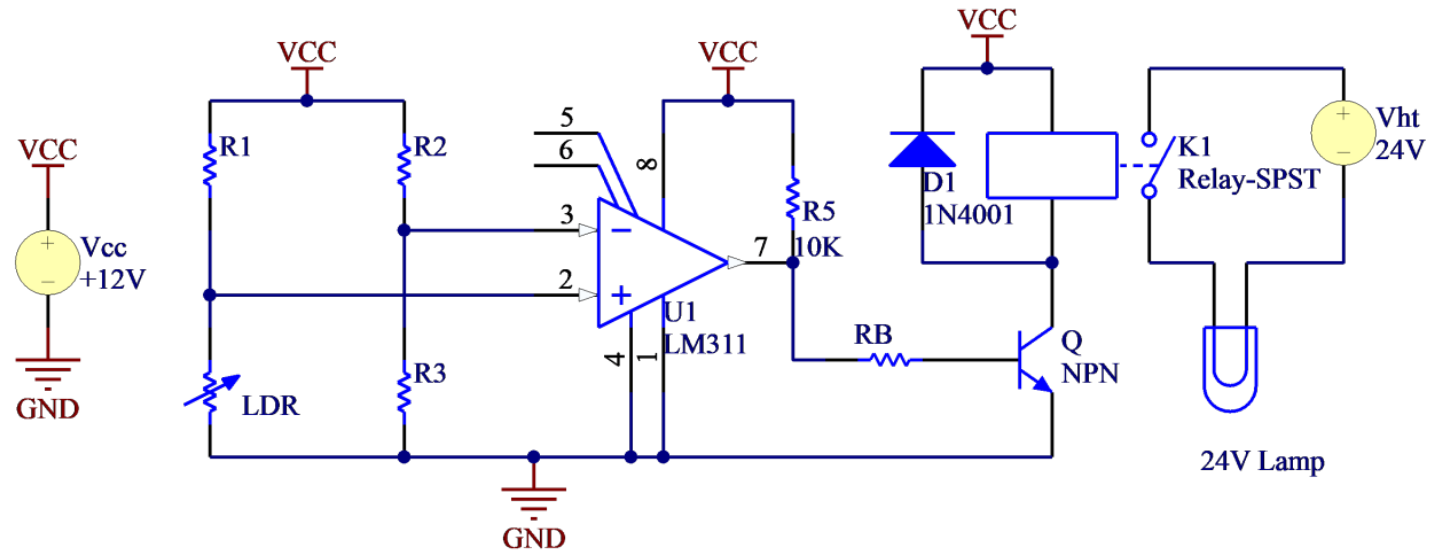
\includegraphics[width=\textwidth]{montage-complet.png}
\caption{Circuit complet du détecteur de pénombre.}
\label{fig:montage-complet}
\end{figure}





\subsection{Étude du transistor}

\Question{
	Comment va se comporter le transistor au cours de la manipulation ?
	Quel est son rôle dans le montage ?
}
{
	Interrupteur permettant d'activer le relais.
}


\Question{
	Pour calculer la valeur de la résistance $R_B$, il faut connaître le gain $\beta$ ou $h_{FE}$ du transistor.
	Déterminez l'expression analytique de $\beta$ en fonction des paramètres du montage présenté en Figure~\vref{fig:npn} et des mesures de tensions $V_i$, $V_{o}$ et $V_{BE}$. Utilisez des résistances $R_C = 1k\Omega$ et $R_B = 100k\Omega$.
}
{
	Gain en courant : $I_C = \beta \cdot I_B$

	On a une maille en sortie : $V_o = V_{CC} - R_C \cdot I_C \Leftrightarrow I_C = \frac{V_{CC} - V_o}{R_C}$.

	Une autre maille en entrée : $V_i - R_B \cdot I_B - V_{BE} = 0 \Leftrightarrow I_B = \frac{V_i - V_{BE}}{R_B}$

	Ainsi $\beta = \frac{I_C}{I_B} = \frac{V_{CC} - V_o}{R_C} \cdot \frac{R_B}{V_i - V_{BE}}$

	$V_{CC} = 12 V$, $R_B = 100k\Omega$, $R_C = 1k\Omega$. $V_i$, $V_o$ et $V_{BE}$ peuvent être mesurées.
}

\Question{
	Réalisez le montage de la Figure~\vref{fig:npn} en appliquant un signal $V_{i}$ triangulaire compris entre 1~V et 2~V et déterminez la valeur précise du $\beta$ de votre transistor.
}
{
	$\sim 500$
}

\begin{figure}[ht]
\centering
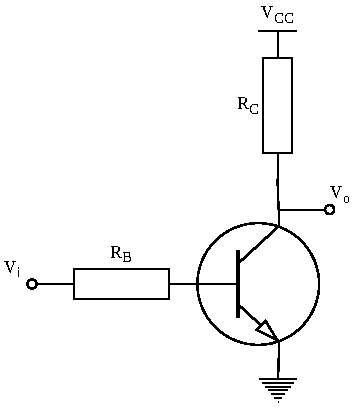
\includegraphics[width=.45\textwidth]{npn-common-emiter.pdf}
\caption{Montage amplificateur à base d'un transistor NPN.}
\label{fig:npn}
\end{figure}


\Question{
	Quelle est la résistance équivalente du relais côté «~contrôle~» ?
}
{
	On utilise le relais \texttt{OJE-SS-112HM}. 
	\texttt{OJE} pour « Miniature PCB Relay OJE, 3kV dielectric between coil and contacts ».
	\texttt{SS} pour « Flux proof », quand on le brase, le flux ne partira pas partout.
	\texttt{1} pour « 1 pôle ».
	\texttt{12} pour les caractéristiques électriques.
	\texttt{HM} pour « 10A type, coil power 450mW~».

	Ses caractéristiques électriques sont les suivantes :
	\begin{itemize}
		\item Rated voltage : 12 VDC
		\item Operate voltage : 8.4 VDC
		\item Release voltage : 0.6 VDC
		\item \textbf{Coil resistance : 320 $\Omega$ ±10\%}
		\item Rated coil power :  450 mW
	\end{itemize}
}

\Question{
	Sur base du montage de la Figure~\ref{fig:montage-complet} et de ce que vous avez trouvé jusqu'à présent, déterminez la valeur de la résistance $R_B$.

	\begin{astuce}
		La résistance $R_5$ connectée à la sortie du \texttt{LM311} sert de \textit{pull-up}. Si on s'intéresse au fonctionnement interne de l'AOP, on voit que sa sortie est prise sur le collecteur du transistor de sortie du montage, d'où l'appellation de «~collecteur ouvert~». Lorsque la sortie du comparateur doit être à l'\textbf{état bas}, le transistor est fermé, connectant le collecteur à l'émetteur qui est connecté à la masse dans notre configuration, \textbf{$V_o = 0$}.
		Par contre, lorsque la sortie du comparateur doit passer à l'\textbf{état haut}, le transistor est ouvert, aucun courant n'entre dans l'AOP et $V_o = V_{CC} - I\cdot R_5$. Si la charge tire peu ou pas de courant, $V_o = V_{CC}$.
	\end{astuce}
}
{
	Il faut bien prendre en compte la résistance $R_5$ dans le calcul de $R_B$. Lorsque l'AOP est à l'état haut, sa sortie est ouverte et aucun courant n'y entre. C'est comme si on connectait VCC et $R_5$ directement à $R_B$ et au NPN.

	On peut procéder de deux façons différentes : considérer le cas limite ou dimensionner un point de fonctionnement précis.

	Dans le premier cas, on va considérer le «~pire~» cas possible, c'est-à-dire lorsque $V_{CE} = 0$ avec un transistor passant. Dans ce cas, sachant que le relais se comporte comme une résistance de collecteur de $320 \Omega$, $I_C$ est maximal et vaut $\frac{V_{CC}}{320 \Omega} = 37.5 mA$.
	En utilisant la valeur de $\beta = h_{FE}$ trouvée précédemment (par exemple 500), on trouve $I_B = \frac{I_C}{\beta} = 75 \mu A$.
	Dans la maille d'entrée, on a $V_{CC} - I_B \cdot (R_5 + R_B) - V_{BE} = 0$, soit $R_B = \frac{V_{CC} - V_{BE} - I_B\cdot R_5}{I_B}$. Avec $V_{CC} = 12 V$, $I_B = 75 \mu A$, $R_5 = 10k\Omega$ et $V_{BE} = 0.6 V$, on a $R_B = 142k\Omega$.
	Il s'agit d'une valeur minimale. En effet, si $V_{CE} > 0$, $I_C$ sera plus faible, donc $I_B$ pourra être plus faible et $R_B$ pour être plus élevée.\\

	On peut aussi trouver une valeur précise sur base de la caractéristique de sortie du transistor, sans faire intervenir son facteur $h_{FE}$.
	On peut tracer la droite de charge du transistor :
	\begin{center}
		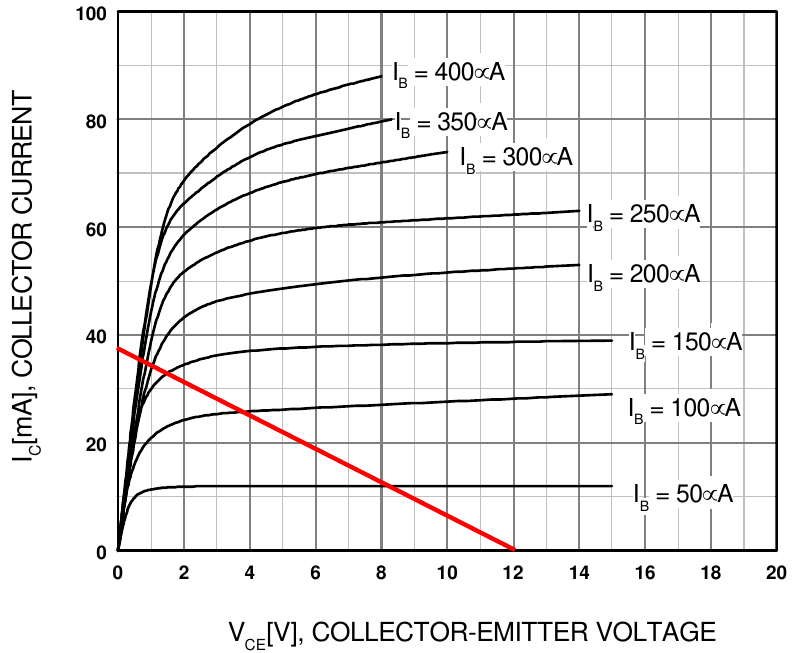
\includegraphics[width=.7\textwidth]{BC546-output-carac.png}
	\end{center}

	On peut notamment avoir un point de fonctionnement à $I_B = 100\mu A$.
	En entrée du transistor, on a comme précédemment $V_{CC} - I_B \cdot (R_5 + R_B) - V_{BE} = 0$, soit $R_B = \frac{V_{CC} - V_{BE} - I_B\cdot R_5}{I_B}$. Avec $V_{CC} = 12 V$, $I_B = 100 \mu A$, $R_5 = 10k\Omega$ et $V_{BE} = 0.6 V$, on a $R_B = 104k\Omega$.

	On peut tout à fait utiliser une résistance de $100 k\Omega$ qui nous donnera un courant $I_B = \frac{V_{CC} - V_{BE}}{R_5 + R_B} = 103.6 \mu A$, toujours un point de fonctionnement valide.\\

	La différence évidente entre les résultats des deux méthodes est due au fait que la caractéristique de sortie tracée dans la datasheet du transistor n'a pas été réalisée pour $h_{FE} = 500$ comme nous l'avons considéré dans la première partie, mais plutôt d'environ 200.
}




\subsection{Étude du relais}
\Question{
	Branchez le côté « bobine » du relais \textit{seul} à l'alimentation de 12~V (n'ajoutez pas le transistor).
	Mesurez la tension à ses bornes lorsque vous éteignez l'alimentation.
	\begin{astuce}
		Préparez la mesure à l'oscilloscope en réglant le \textit{trigger} sur un flanc descendant à une tension de 5~V et appuyez enfin sur le bouton « Single » afin de ne capturer qu'un seul événement sur lequel vous pourrez vous attarder. 

		Retirez le fil d'alimentation $V_{CC}$ de la breadboard afin de simuler une coupure brusque de l'alimentation.
	\end{astuce}
	Quel phénomène observez-vous ?
}
{
	La configuration de l'oscilloscope est essentielle pour que la prise de mesure soit correcte.
	Sur-tension au moment où on coupe l'alimentation.
	\begin{center}
		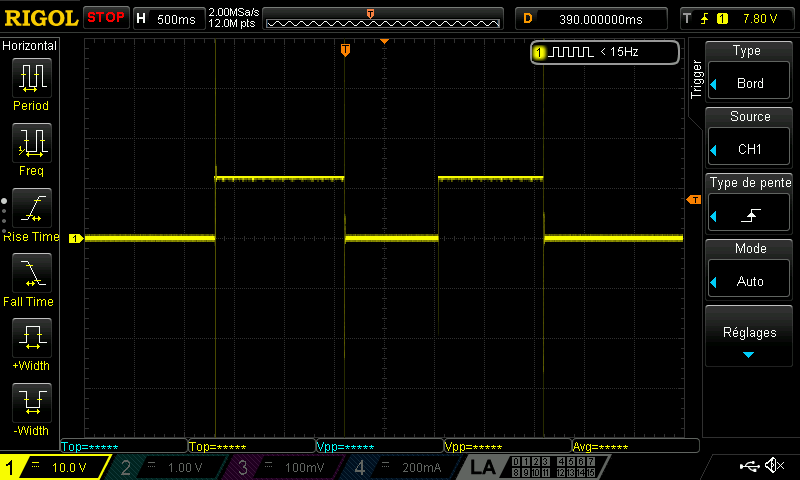
\includegraphics[width=.8\textwidth]{DS1Z_QuickPrint2.png}\\
		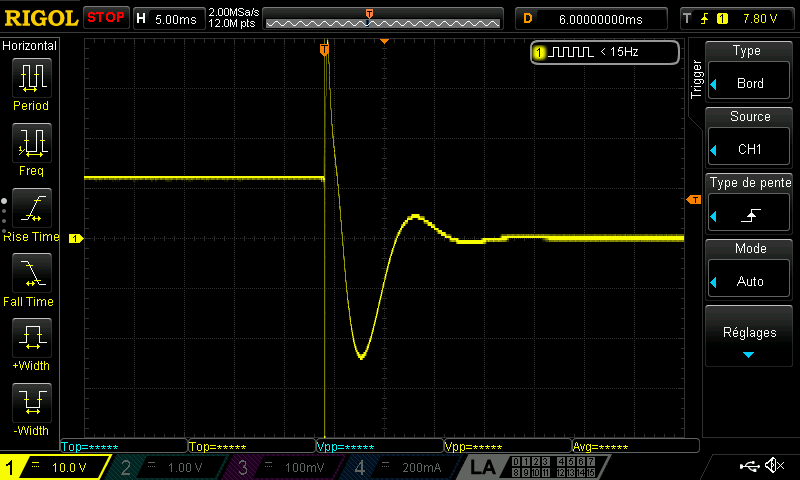
\includegraphics[width=.8\textwidth]{DS1Z_QuickPrint1.png}
	\end{center}
}


\Question{
	Ajoutez la diode de \textit{flyback} comme indiqué sur le schéma\footnote{Ce dernier fait mention d'une diode 1N4001. Vous pouvez utiliser n'importe quelle diode 1N400x, comme la 1N4007. Elles ont toutes la même caractéristique à l'exception des tensions maximales supportées qui sont meilleures pour les valeurs de «~x~» plus élevées.} et répétez l'expérience.
	Quelle différence observez-vous ?
	Qu'en concluez-vous sur l'utilité de la diode ?
}
{
	Pic atténué, la diode protège le NPN pilotant le relais.
	\begin{center}
		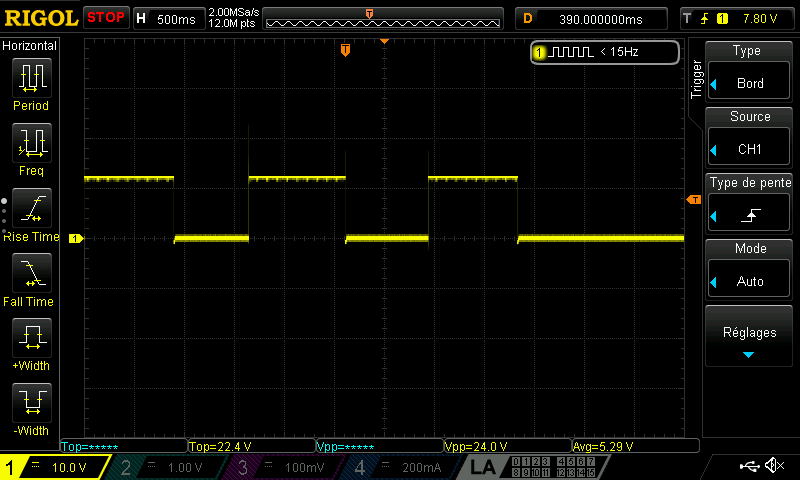
\includegraphics[width=.8\textwidth]{DS1Z_QuickPrint3.png}\\
		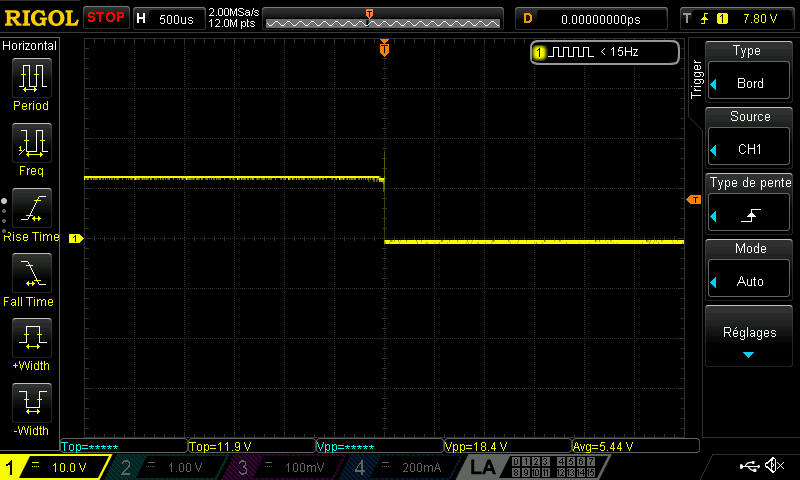
\includegraphics[width=.8\textwidth]{DS1Z_QuickPrint4.png}
	\end{center}
}








\subsection{Étude de la LDR et du comparateur}

\Question{
	Quelle est la valeur de la LDR illuminée et dans l'obscurité ?
}
{
	\begin{itemize}
		\item Dans l'obscurité : $22 k\Omega$ avec seulement sa main au-dessus, $20 M\Omega$ dans l'obscurité complète.
		\item Luminosité ambiante : $1.6 k\Omega$
		\item Luminosité directe : $< 100\Omega$
	\end{itemize}

	La valeur de la résistance augmente si la luminosité diminue.
}

\Question{
	Dimensionnez les résistances $R_1$, $R_2$ et $R_3$ afin de répondre au cahier des charges.
}
{
	On veut que la lampe s'allume si la luminosité est trop basse.
	Sachant que si la luminosité \textit{baisse}, la résistance \textit{augmente}, ça veut donc dire que la tension $V_+$ va \textit{augmenter}.

	On a $V_+ = V_{CC} \cdot \frac{LDR}{R_1 + LDR}$ et $V_- = V_{CC} \cdot \frac{R_3}{R_2+R_3}$.

	Le but est qu'à basse luminosité, $V_+ > V_-$.

	Prenons par exemple $R_1 = 10k\Omega$, ce qui nous donne un $V_+$ variant entre 1.52 V (luminosité ambiante, $LDR \approx 1.6k\Omega$) et 8.25 V (main couvrante, $LDR = 22k\Omega$).

	Dès lors, il faut que $V_-$ soit comprise entre ces deux seuils, par exemple avec $R_3 = 2.2k\Omega$ et $R_4 = 3.3 k\Omega$, on obtient $V_- = 7.2 V$.
}

% \Question{
% 	L'AOP utilisé dans le montage, le LM311, propose un système de compensation de sa tension de décalage (offset). Trouvez où se trouve l'information sur son utilisation dans la datasheet de Texas Instruments.
% }
% {
% 	p.15 de la datasheet du LM311.
% }

% \Question{
% 	En utilisant le LM311 \textit{seul}, observez à l'oscilloscope l'amplitude de sa tension de décalage. Est-ce cohérent avec les valeurs 
% 	Réfléchissez au signal à envoyer dans les entrées de l'AOP pour réaliser ce test.
% }
% {
% 	Pour mesurer la tension de décalage en sortie, il ne faut rien envoyer au montage, mais il ne faut pas laisser les entrées flottantes pour autant. Normalement, il faudrait les connecter au montage en court-circuitant les alimentations, mais dans notre cas on peut simplement les connecter à la masse.

% 	La tension de décélage en entrée devrait être comprise entre 2 et 7.5mV. Comme on travaille en boucle ouverte, il va peut-être falloir la compenser.
% }

% \Question{
% 	À l'aide d'un potentiomètre de $xxx k\Omega$, réalisez le montage de compensation (\textit{balance}) afin d'annuler cette tension de décalage.
% }
% {}





\subsection{Assemblage du montage complet}

\Question{
	Quel est le comportement attendu du montage complet ?
}
{
	Si la LDR est dans l'obscurité, la lampe s'allume, sinon elle s'éteint.
}

\Question{
	Réalisez le montage complet sur breadboard et vérifiez son bon fonctionnement.
}
{

}

% \Question{

% }
% {

% }

% \begin{astuce}
% \end{astuce}

\end{document}
